\chapter{PROPOSED SYSTEM}

\paragraph{}
The proposed system turns the one-way pipeline of the first version into a Lambda architecture whose storage tier is sharded, replicated, backed up and recoverable from an immutable lake.

\section{Description of Proposed System}

\paragraph{}
Figure~\ref{Fwk1} shows the architecture. A producer replays CSV records into Kafka, keyed by flow so that the four partitions receive equal load. Spark Structured Streaming is the \emph{speed layer}: it classifies each micro-batch and writes it twice. The \emph{hot} copy (alerts and metrics) goes to the sharded MongoDB cluster that serves the dashboard; the \emph{cold} copy (every event) is appended to the Parquet lake, the immutable master dataset. The \emph{batch layer} runs Spark SQL over the lake and stores pre-computed views in MongoDB; the dashboard reads both. A backup manager snapshots MongoDB, the streaming checkpoints and the lake.

\begin{figure}[H]
\centering
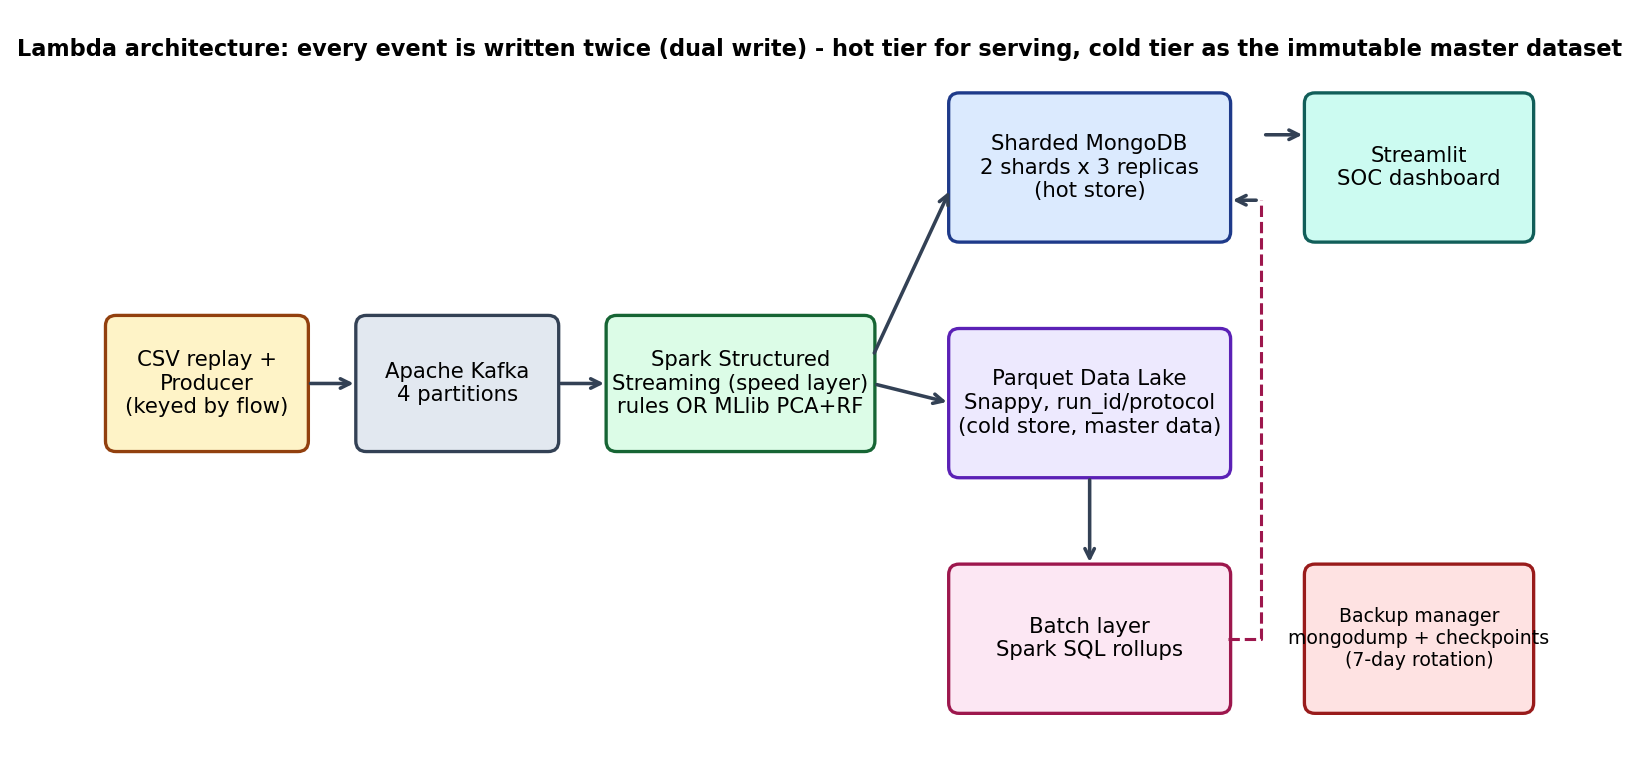
\includegraphics[width=\textwidth]{images/Framework.png}
\caption{Lambda architecture of the proposed system}
\label{Fwk1}
\end{figure}

\paragraph{}
\textbf{Modules.} (1) \emph{Producer}: reads the CSV, builds JSON, selects a partition key. (2) \emph{Detector}: four metadata rules plus a PCA(32) + Random Forest model on the payload; hybrid verdict is the logical OR. (3) \emph{Sinks}: idempotent MongoDB upserts and the Parquet lake writer. (4) \emph{Sharded storage}: described below. (5) \emph{Batch analytics}. (6) \emph{Backup and recovery}. (7) \emph{Dashboard}.

\section{Sharding and replication: the storage design}
\paragraph{}
The alert collection is write-heavy and grows without bound, so it is \emph{sharded}; each shard is a three-member \emph{replica set}, so that one node can fail without data loss (Figure~\ref{DP1}). A \texttt{mongos} router hides the shards from clients, so the pipeline needs only a different connection string. The config server stores which hash range lives on which shard.

\begin{figure}[H]
\centering
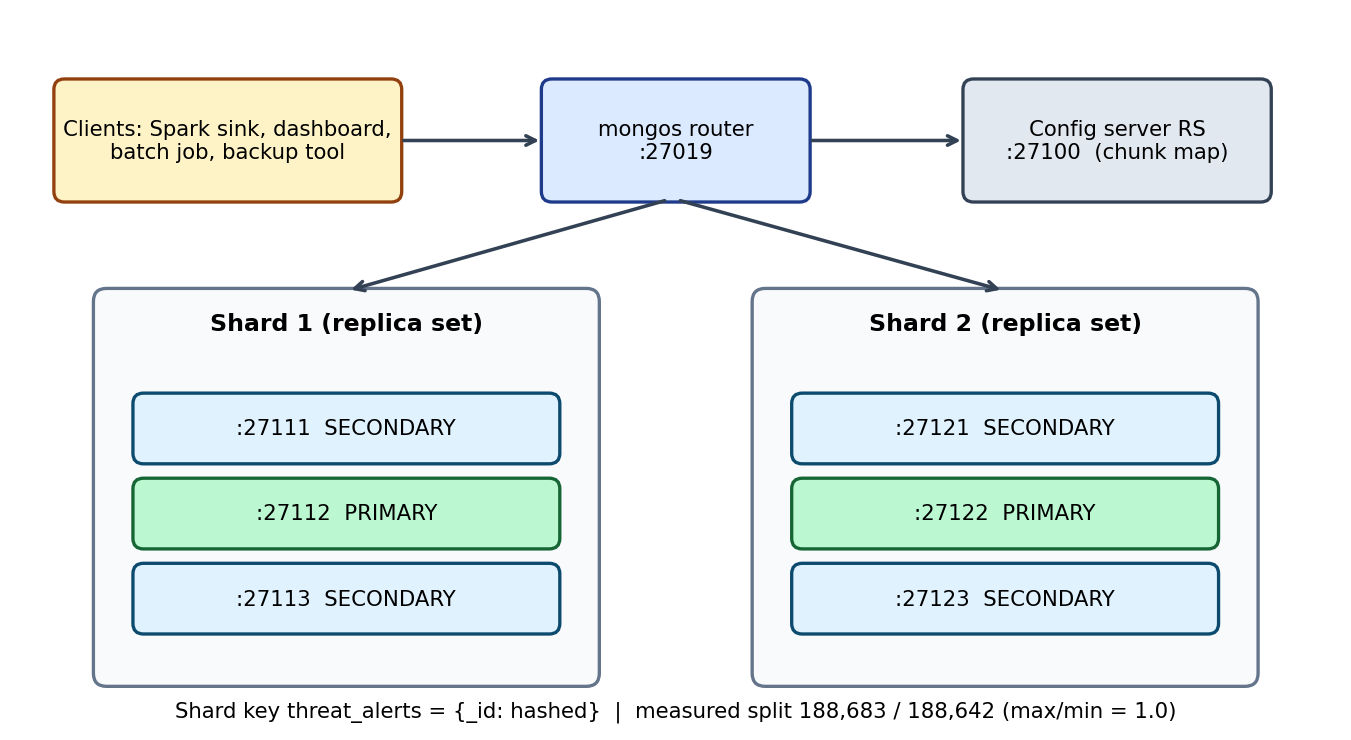
\includegraphics[width=0.95\textwidth]{images/DP1.png}
\caption{Sharded and replicated MongoDB cluster (2 shards $\times$ 3 replicas)}
\label{DP1}
\end{figure}

\begin{table}[H]
\centering
\begin{tabular}{|p{3.6cm}|p{3.6cm}|p{6.2cm}|}
\hline
\textbf{Collection} & \textbf{Shard key} & \textbf{Reason} \\ \hline
\texttt{threat\_alerts} & \texttt{\{\_id: hashed\}} & \texttt{\_id} is \texttt{topic:partition:offset}, which only grows; a ranged key would send all inserts to one hot shard. Idempotent upserts by \texttt{\_id} hit exactly one shard. \\ \hline
\texttt{historical\_ threat\_rollups} & \texttt{\{run\_id, rollup\_type\}} & Always read by run and type, so reads are targeted range queries. \\ \hline
\texttt{batch\_metrics} & not sharded & Tiny; sharding would add routing cost only. \\ \hline
\end{tabular}
\caption{Shard-key decisions}
\end{table}

\section{Why sharding with replication, and not a replica set alone}
\paragraph{}
Replication and sharding solve different problems. A replica set has a single primary that takes every write and holds a full copy of the data on each node; it protects against a server crash but neither splits write load nor lets the data set grow beyond one machine. Sharding splits the data and the writes across shards. Production shards are themselves replica sets, so the design is the combination taught in the course: sharding for scale, replication for availability. We chose it because the alert collection is the growing, write-heavy part of the system, because streaming means many parallel writers, and because it requires no code change in the pipeline. Neither mechanism protects against deletion, since replicas copy a mistaken delete within milliseconds; that is why snapshots and the lake exist.

\section{Four layers of data protection}
\begin{table}[H]
\centering
\begin{tabular}{|p{1cm}|p{4.2cm}|p{7.8cm}|}
\hline
\textbf{\#} & \textbf{Layer} & \textbf{Failure handled} \\ \hline
1 & Sharding + replication & A database server crashes: survivors elect a new primary \\ \hline
2 & Verified snapshot backups & The database is deleted or corrupted \\ \hline
3 & Parquet data lake & Database and every backup are lost: rebuild from the lake \\ \hline
4 & Checkpoints inside snapshots & The streaming job restarts without re-reading or skipping Kafka data \\ \hline
\end{tabular}
\caption{Layers of protection}
\end{table}

\section{Description of Target Users}
\paragraph{}
Security-operations analysts who need current alerts and historical trends, and platform operators who must keep the data safe and recover it. The design principles applied are \emph{redundancy} (replicas), \emph{immutability} (append-only lake), \emph{idempotence} (deterministic document identifiers) and \emph{separation of concerns} (detection logic is independent of storage).

\section{Advantages/Applications of Proposed System}
\paragraph{}
Advantages: survives node failure with no data loss; recoverable from deletion and from loss of all backups; scales out by adding shards; detects application-layer attacks missed by the rules; batch analytics are cheap because they use a columnar lake. Applications include network security monitoring, any log or telemetry pipeline, and teaching Big Data storage trade-offs.

\section{Scope (Boundary of proposed system)}
\paragraph{}
The system replays historical data rather than capturing live packets. All components run on one laptop, so the cluster demonstrates correct distribution, routing and failover but not throughput gains or protection against loss of the machine; off-site copies of the backups and the lake are outside the scope (Chapter~8).
